\documentclass[12pt,twoside,book]{article}

\usepackage{epsf}
\usepackage{amsmath,amssymb}
\usepackage{slashed}

\usepackage[dvipdfmx]{graphicx,hyperref}
\usepackage{ascmac}
\usepackage{braket}
\usepackage{multirow}
\usepackage{cite}
\usepackage[titletoc]{appendix}

\hypersetup{% hyperref option list
setpagesize=false,
 bookmarksnumbered=true,%
 bookmarksopen=true,%
 colorlinks=true,%
 linkcolor=blue,
 citecolor=red,
}

\usepackage{titlesec}
\usepackage{picture}
\usepackage{ulem}
\usepackage{fancyhdr}
\usepackage{tikz}
\usetikzlibrary{%
   decorations.fractals%
  ,decorations.pathmorphing%
  ,shadows%
  }

\usepackage{colortbl}
\usepackage{comment}
\usepackage{bm}

\setlength{\textwidth}{16.5cm}
\setlength{\textheight}{21.5cm}
\setlength{\oddsidemargin}{30truemm}
\addtolength{\oddsidemargin}{-1truein}
\setlength{\evensidemargin}{20truemm}
\addtolength{\evensidemargin}{-1.2truein}
\setlength{\topmargin}{0cm}
\setlength{\footskip}{1cm}

\makeatletter
\newcommand{\figcaption}[1]{\def\@captype{figure}\caption{#1}}
\newcommand{\tblcaption}[1]{\def\@captype{table}\caption{#1}}
\makeatother

\makeatletter
  \renewcommand{\theequation}{%
  \thesection.\arabic{equation}}
  \@addtoreset{equation}{subsection}
\makeatother

\renewcommand{\arraystretch}{1.2}
\renewcommand{\topfraction}{1.0}
\renewcommand{\bottomfraction}{1.0}
\renewcommand{\baselinestretch}{1.1}

%%%%%%%%%%%%%%%%%%%%%%%%%%%%%%%
%%%    remove the following commands when finalizing
%%%%%%%%%%%%%%%%%%%%%%%%%%%%%%%
\def\rem#1{ {\bf\textcolor{red}{($\clubsuit$ #1 $\clubsuit$)}}}
%%%%%%%%%%%%%%%%%%%%%%%%%%%%%%%
%%%%%%%%%%%%%%%%%%%%%%%%%%%%%%%

\newenvironment{titlelineskip}{
\baselineskip=12mm
}

\makeatletter
\def\ps@fancy{%
\def\sectionmark##1{\markboth{\ifnum \c@secnumdepth>\z@ Section \thesection . \hskip 1em\relax \fi ##1}{}}%
% \def\chaptermark##1{\markboth{\ifnum \c@secnumdepth>\z@ \thechapter\hskip 0.5em\relax \fi ##1}{}}%
\def\subsectionmark##1{\markright {\ifnum \c@secnumdepth >\@ne \thesubsection \hskip 1em\relax \fi ##1}}%
% \def\sectionmark##1{\markright {\ifnum \c@secnumdepth >\@ne \thesection\hskip 0.5em\relax \fi ##1}}%
\ps@@fancy
\gdef\ps@fancy{\@fancyplainfalse\ps@@fancy}%
\ifdim\headwidth<0sp
\global\advance\headwidth123456789sp\global\advance\headwidth\textwidth
\fi
}
\makeatother

\pagestyle{fancy}
\fancyhead{}
\fancyhead[RO,LE]{\small\thepage}
\fancyhead[CO]{\rightmark}
\fancyhead[CE]{\leftmark}
\fancyfoot{}
\renewcommand{\headrulewidth}{0.4pt}

\allowdisplaybreaks[1]

\DeclareSymbolFont{lettersA}{U}{txmia}{m}{it}
\DeclareMathSymbol{\RRR}{\mathord}{lettersA}{'222}

\begin{document}

\newcommand{\lsim}{\stackrel{<}{_\sim}}
\newcommand{\gsim}{\stackrel{>}{_\sim}}

\renewcommand{\thefootnote}{$\natural$\arabic{footnote}}
\setcounter{footnote}{0}

% Section
\titleformat{\section}[display]
  {\LARGE\fillast\bfseries}
  {Section \thesection}
  {1ex minus .1ex}
  {\LARGE\bf}
  \titlespacing{\section}
  {3pc}{*3}{*2}[3pc]

\begin{titlepage}

\begin{center}
 
\begin{titlelineskip}

\vskip .75in

{\Large \it

 Ph.D. Thesis

}

\vskip 1.0in

{\Huge \bf

 Indirect study of electroweakly\\
 interacting particles\\
 at 100 TeV hadron colliders

}

\vskip .75in

{\Large 
So Chigusa
}\\

{\Large \it Department of Physics}

\vfill

\begin{figure}[h]
 \begin{center}
  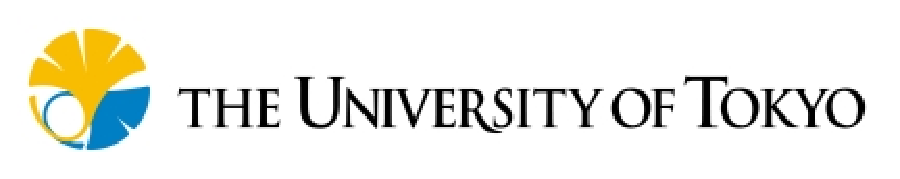
\includegraphics[width=0.6\hsize]{figure/univ.eps}
 \end{center}
\end{figure}

\vskip 0.35in

{\Large December 2019}

\end{titlelineskip}

\end{center}

\vspace{0.5in}

\end{titlepage}

\thispagestyle{empty}

\vspace*{1.50in}

\begin{abstract}
 \rem{To be written}
\end{abstract}

\clearpage

\thispagestyle{empty}

\vspace*{.75in}

{\LARGE \bf
Acknowledgments
}

\vskip .50in

\rem{To be written}

% I would like to thank my supervisor, Takeo Moroi, who provided
% stimulating discussions, helpful comments, fruitful suggestions and
% collaboration.  I am also grateful to Koichi Hamaguchi, Kazunori
% Nakayama, Natsumi Nagata and all the members of the particle physics
% group at the University of Tokyo for their hospitality.  My work is
% supported by the Program for Leading Graduate Schools, MEXT, Japan.
% Finally, I would like to express my gratitude to my family, friends and
% all things which allow me to enjoy studying physics.

\clearpage

\thispagestyle{empty}

\tableofcontents

\clearpage

\renewcommand{\thepage}{\arabic{page}}
\setcounter{page}{1}

\section[Introduction]{Introduction}
\setcounter{equation}{0}

\vskip 0.1in

\rem{Unit: $\hbar=c=k_B=1$}

\rem{Definition of ``SM''}

\rem{Definition of ``WIMP''}

\section[Weakly interacting massive particles]{Weakly interacting
 massive particles}
\setcounter{equation}{0}

\vskip 0.1in

\subsection[WIMPs as a dark matter candidate]{WIMPs as a dark matter candidate}

One of the most important evidences of the beyond SM is the existence
of dark matter (DM) \cite{Zwicky:1933}.  DM is an unknown object that
occupies a non-negligible ratio of the total energy of our universe,
but has not yet been directly observed because of its weak interaction
with the SM particles.\footnote{
%%
At worst DM interacts with the SM particles through the gravity, which
is considerably weaker than all the other known interactions.
\rem{Mention to Ema paper??}
}
%%
In spite of its invisibility, the existence of DM is confirmed by
several astrophysical observations such as the mass measurement using
the gravitational lensing effect caused by galaxies and clusters
\cite{Zwicky:1937, Trimble:1987ee}, the flatness of galactic rotation
curves further the optical radius \cite{1939LicOB..19...41B,
Begeman:1991iy}, the measurement of the power spectrum of the cosmic
microwave background (CMB), and so on.  In particular, the observation
of CMB allows us the precise determination of various cosmological
parameters \cite{Jungman:1995av, Jungman:1995bz} including the density
of the non-relativistic matter and baryon, which is currently
determined as \cite{Aghanim:2018eyx}
\begin{align}
 \Omega_m h^2 &= 0.1430 \pm 0.0011,\\
 \Omega_b h^2 &= 0.02237 \pm 0.00015,
\end{align}
where $h \sim \mathcal{O}(1)$ is the Hubble constant in units of
$100\, \mathrm{km}\, \mathrm{s}^{-1}\, \mathrm{Mpc}^{-1}$.  The
difference between $\Omega_m h^2$ and $\Omega_b h^2$ implies the
existence of DM and its abundance $\Omega_\chi h^2 \simeq 0.12$.

In cosmology, DM production mechanisms that try to explain the DM
abundance are divided into two main categories: thermal and
non-thermal production.  The former assumes the equilibrium between
the DM and the thermal bath in the early universe.  As the universe
expands, the interaction rate that maintains the thermal equilibrium
becomes smaller and the DM decouples from the thermal bath at some
time, which is the so-called \textit{freezeout}.  As we will see
below, the resulting abundance of the DM in this scenario is mainly
controlled by the temperature of the thermal bath $T_f$ when the
freezeout occurs.  On the other hand, non-thermal production assumes
the DM production by some processes irrespective of the thermal bath
such as decay of a heavy particle.  Since the thermal production
scenario can be realized in relatively simple setup and WIMPs are well
motivated in connection with this kind of scenario, we focus on it.

We assume the stable DM particle $\chi$ with mass $m_\chi$ can pair
annihilate into SM particles with some cross section $\sigma$.  When
DM is in thermal equilibrium with the thermal bath of temperature $T$,
DM has some fixed velocity distribution.  \rem{More clearly}  Let $v$
be the relative velocity of annihilating DM particles and
$\Braket{\sigma v}$ be the thermal average of the product of $\sigma$
and $v$.  By using this quantity, we can write down the Boltzmann
equation for the DM number density $n$ as
\begin{align}
 \frac{d (n a^3)}{d t} =
 - (n^2 - n_{\mathrm{eq}}^2) a^3 \Braket{\sigma v},\label{eq_boltzmann}
\end{align}
where $t$ and $a$ are the time coordinate and the scale factor of the
Friedmann Robertson Walker metric
\begin{align}
 d s^2 = - d t^2 + a(t)^2 d \bm{x}^2,
\end{align}
while $n_{\mathrm{eq}}$ denotes the number density of DM in
equilibrium.

Here we assume that the freezeout occurs when the relativistic
radiation dominates the total energy of the universe, which will be
verified to be correct later.  Then we can use the Einstein equation
together with the knowledge of thermodynamics to derive $a \propto
T^{-1}$ and
\begin{align}
 d t = -2 \sqrt{\frac
 {3}{16\pi G g_{*} a_B}} \frac{d T}{T^3},
\end{align}
with $G$ and $a_B$ being the gravitational constant and the
coefficient of the Stefan-Boltzmann law.  $g_{*}$ represents the
effective degrees of freedom of relativistic particles in the thermal
bath
\begin{align}
 g_{*} \equiv \sum_{\mathrm{bosons}} g_B +
 \frac{7}{8} \sum_{\mathrm{fermions}} g_F,
\end{align}
where both $g_B$ and $g_F$ denote the spin degrees of freedom of each
particle in the summation.  Finally, by defining dimensionless
parameters $x \equiv T / m_\chi$ and $u(x) \equiv n / T^3$ and
substituting $a_B = \pi^2 / 15$, Eq.~\ref{eq_boltzmann} is deformed as
\begin{align}
 test
\end{align}

\begin{appendices}
 
\end{appendices}

\clearpage

\bibliographystyle{elsarticle-num}
\bibliography{phd}

\end{document}
